\documentclass{subfiles}
\begin{document}

\section{Time evolution}\label{sec:time_evolution}
The time evolution of a quantum system is described by the Time-Dependent Schrödinger Equation (TDSE) \eqref{eq:tdse}. The TDSE shows the behaviour of a quantum system over time under the influence of the system Hamiltonian. While simple systems without time-dependence admit closed-form solutions, most physically realisable systems - especially those relevant for quantum control and information - exhibit time-dependent behaviou, and is generally not exactly solvable analytically. Treating such systems that cannot be solved analytically, require numerical methods to approximate the systems evolution. Understanding time evolution is crucial for modelling driven systems such as qubit under external control field, where energy transitions reveal non-trivial dynamics\cite{landau1932theorie, zener1932non}, or simulating quantum gates in quantum computing \cite{leinonen2024coulomb, nazir2005anticrossings}. In this section, we outline the framework for quantum time evolution and introduce the time-evolution operator, which is at the heart of quantum dynamics, and the basis for our numerical methods. We will also conceptualize the steps behind the numerical framework for solving the time-dependent Schrödinger equation, and also for discretizing the time evolution operator. \\
\subsection{Time evolution operator}
Simulating the dynamics of any quantum system is seen through the evolution of the quantum mechanical state representing the system at hand. The time evolution of a quantum state from time $t_0$ to $t$ is expressed by the linear unitary time-evolution operator $U(t, t_0)$, which is a solution to the time-dependent Schrödinger equation \eqref{eq:TDSE}\cite{sakurai1986modern, berera2021quantum}. This operator should do the following
\begin{equation}
    \ket{\Psi(t)} = U(t, t_0)\ket{\Psi(t_0)}
\end{equation}
and it must satisfy the following critera:
\begin{itemize}
    \item \textbf{Unitarity:} $U(t, t_0)U^\dagger(t, t_0) = U^\dagger(t, t_0)U(t, t_0) = \mathbb{I}$, meaning it preserves the norm of the quantum mechanical state.
    \item \textbf{Composition property:} $U(t_2, t_0) = U(t_2, t_1)U(t_1, t_0)$, meaning the time-evolution operator is a composition of smaller time-evolution operators that are time-ordered ($t_2>t_1>t_0$).
    \item \textbf{Continuity:} $\lim_{dt\to 0}U(t_0 + dt, t_0) = \mathbb{I}$, meaning the time-evolution operator is continuous, and reduces to identity when the time difference is zero.
\end{itemize}
All these critera can be satisfied by 
\begin{align*}
    U(t_0 + dt, t_0) = 1 - i\Omega(t_0) dt,
\end{align*}
where $\Omega$ is a Hermitian operator, and $dt$ is the infinitesimal time difference. The 3rd criteria is satisfied naturally as $dt$ goes to zero, while the 1st and 2nd criteria is satisfied to first order 
\begin{align*}
    U^\dagger(t_0 + dt, t_0)U(t_0 + dt, t_0) = (1 + i\Omega(t_0)^\dagger)(1 - i\Omega(t_0)) = 1 + \mathcal{O}(dt^2) \approxeq 1
\end{align*}
and
\begin{align*}
    &U(t_0 + 2dt, t_0) = 1 - i2\Omega(t_0)dt, \\
    &U(t_0 + 2dt, t_0 +dt)U(t_0 + dt, t_0) = 1 - 2i\Omega(t_0)dt + \mathcal{O}(dt^2),
\end{align*}
if we have a small enough time-step $dt$, where we can safely ignore higher order terms. But how to identify the operator $\Omega$? We identify from classical mechanics that the Hamiltonian operator is the propagator of the system \cite{sakurai1986modern} 
\begin{align*}
    \Omega = \frac{H}{\hbar}.
\end{align*}
Which means that the time-evolution operator can be expressed as 
\begin{align*}
    U = 1 - \frac{i}{\hbar}Hdt,
\end{align*}
which we can see is the first order approximation of the exponential series
\begin{align*}
    e^{\frac{-i}{\hbar}Ht} = 1 - \frac{i}{\hbar}Ht + \frac{1}{2!}\bigg(\frac{-i}{\hbar}Ht\bigg)^2 + ... .
\end{align*}
This is the full form of the time-evolution operator, often coined time-propagator, and is given by
\begin{equation}
    U(t, t_0) = \mathcal{T}\text{exp}\bigg(\frac{-i}{\hbar}\int_{t_0}^t H(t')dt'\bigg)\label{eq:time_evolution_operator},
\end{equation}
where the integral must be time-ordered, and swapped with the Dyson series expansion should the Hamiltonian be time-dependent, and non-commutative at different times (see chapter 2.1.2 in \cite{sakurai1986modern}). For a time-independent Hamiltonian $H$, the time-evolution operator simplifies to 
\begin{align*}
    U(t, t_0) = e^{-\frac{i}{\hbar}H(t-t_0)},
\end{align*}
allowing for analytical propagation of the system. In contrast, the time-dependent case \eqref{eq:time_evolution_operator} requires numerical treatment to solve the integral, as the exponential cannot be solved analytically. 

\subsection{Numerical time propagation}
The time-propagator in \eqref{eq:time_evolution_operator} involves a time-ordered exponential, which generally cannot be solved analytically for a time-dependent Hamiltonian $H(t)$. Therefore, we must look to numerical methods to approximate the integral. Choice of method is crucial, and it depends on desired accuracy, computational cost and stability. There are some other criteria to consider when developing, or choosing, a numerical method for time propagation. The method should preserve the norm of the wavefunction, and it should preserve the unitarity of the time-evolution operator. 
\\

To simulate time evolution of a quantum system numerically, we start by discretizing time $t$, into smaller intervals (time steps) $\Delta t$. Doing so allows us to approximate the time-evolution operator as a product of smaller time-evolution operators, which can be solved iteratively (recall the composition property of the time-evolution operator). At each step then, the wavefunction is evolved by approximating the true time-evolution operator on the time interval $[t, t+\Delta t]$. \\ 

The simplest approximative method is the \emph{Euler-Cromer} method, a first order method given by Taylor expansion of the time-evolution operator
\begin{align}
    U(t + dt, t) = 1 - \frac{i}{\hbar}H(t)dt\label{eq:euler_cromer},
\end{align}
which leads to an explicit update of the wavefunction as 
\begin{align*}
    \ket{\Psi(t + dt)} = \bigg(1 - \frac{i}{\hbar}H(t)dt\bigg)\ket{\Psi(t)}.
\end{align*}
This is a simple and fast, but inaccurate method. While this method is simple to implement and computationally inexpensive, it suffers from numerical instability and is not unitary nor norm-preserving. This means that the wavefunction will not be normalized after each time step, and the norm of the wavefunction will diverge over time, and we may obtain non-physical results should we want to evolve for longer timespans. \\ 
% Matrix exponentiation
To improve the accuracy and stability of time propagation, higher-order and norm-preserving methods are generally preferred. One straightforward approach is to compute the matrix exponential of the Hamiltonian over each time step. Since this operator is unitary by construction, it ensures that the wavefunction remains normalized and the dynamics remain physically consistent. This method is particularly appealing for low-dimensional systems, where the Hamiltonian can efficintly be diagonalized, and the matrix exponential can be computed. \\

In practice, this matrix exponential is compututed on a discretized time interval by the expression
\begin{equation}
    U(t + dt, t) = e^{-\frac{i}{\hbar}H(t)\Delta t}\label{eq:numerical_time_evolution_operator},
\end{equation}
assuming that the Hamiltonian is approximatively constant over the time interval $\Delta t$. \\

This naturally is an exact update rule for time-independent Hamiltonians, but the accurateness of this method depends on the size of the time step $\Delta t$ and how the Hamiltonian varies over the time intervals. This does however introduce a new alley for approximations, where we may introduce various methods to approximate the Hamiltonian over the time interval, such as the mid-way approximation, where we assume a better approximation is the average of the Hamiltonian at the start and end of the time interval, i.e
\begin{align*}
    U(t + dt, t) = e^{-\frac{i}{\hbar}\frac{H(t) + H(t + dt)}{2}\Delta t}.
\end{align*}
Further on, we will explore more such ways to approximate the time-evolution operator, and in this work we shall investigate how these different approximations affect the time-evolution of our coupled double Morse potential system.\textcolor{red}{TODO: Will we? Or remove if we do not.} \\ 

% Numerical integrations
Direct matrix exponentiation, however, quickly becomes intractable for most computers, as the system increases, due to the computational burden of diagonalizing, or exponentiating, large matrices - commonly referred to as \emph{the curse of dimensionality}, for the exponential increase in computational cost as we increase the dimension of our system. For this reason, it is often more efficient to apply numerical integration methods. A range of numerical integration methods can be applied to evolve the quantum wavefunction, each with its own advantages and disadvantages. These methods generally involve discretizing time and updating the wavefunction iteratively by approximating the time-evolution operator over small time intervals. While these methods are generally more computationally efficient than direct matrix exponentiation, they may not preserve unitarity exactly - however, many such methods can be made to do so approximatively. Most of these methods build upon Taylor expansions, as in the simple case of the Euler-Cromer method shown in \eqref{eq:euler_cromer}, and more complex methods can be seen as higher-order approximations of the time-evolution operator. 
\\

Despite these limitations, numerical integration methods are widely used in quantum dynamics simulations, and they can provide accurate results for a wide range of systems. In this work, we will explore matrix exponentiation as a baseline method for time propagation, and we will compare it to other numerical integration methods. This will allow us to assess the accuracy and efficiency of other approaches for simulating quantum dynamics in our system. 
\\

Returning to our simple system \eqref{eq:landau_zener}, the time-evolution of a two-level system under a time-varying Hamiltonian is illustated in figure \ref{fig:landau_zener}, where the population transfer between the two first energy eigenlevels $\phi_0 = \ket{0}$ and $\phi_1=\ket{1}$, and avoided crossing reflect the dynamics driven by the time-evolution operator applied using direct matrix exponentiation. In figure \ref{fig:landau_zener}, we highlight how some of the simplest methods diverge when evolving the simple system previously introduced in section \ref{sec:avoided_crossings}.
\begin{figure}[h!]
    \centering
    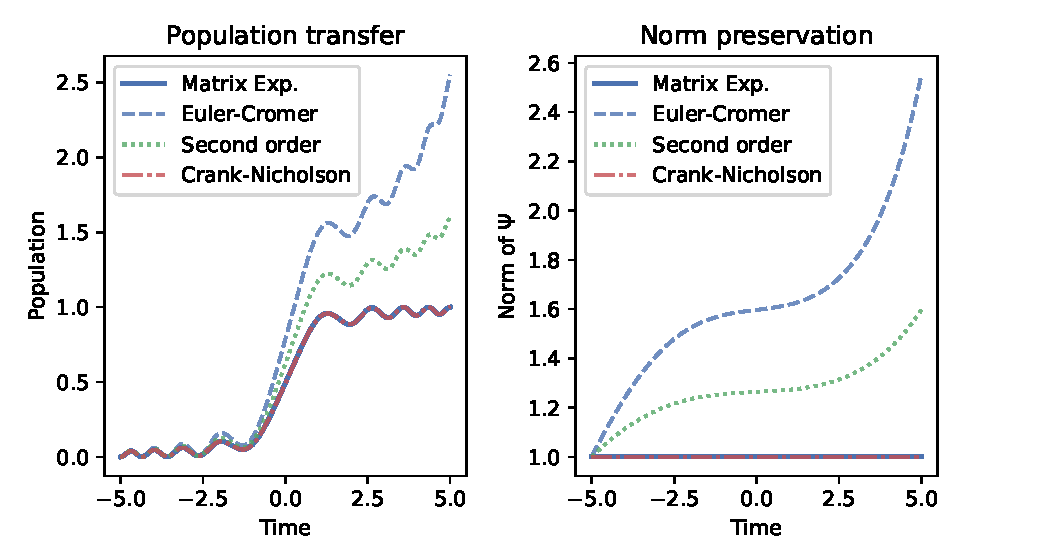
\includegraphics[width=1.0\textwidth]{figs/landau_zener_numerical_methods.pdf}
    \caption{Time evolution of a two-level system under a time-varying Hamiltonian. Population transfer between $\ket{0}$ and $\ket{1}$ and wavefunction norm are shown, demonstrating how the simpler Euler-Cromer and second-order symmetric methods deviate from the exact solution, while Crank-Nicolson remains both norm-preserving and more accurate, and overlaps well with the exact direct matrix exponentiation.}\label{fig:landau_zener}
\end{figure}
\end{document}